\documentclass[aspectratio=169]{beamer}

\usetheme{default}
\setbeamertemplate{navigation symbols}{}
\setbeamertemplate{itemize item}{\color{black}\textbullet}
\setbeamertemplate{itemize subitem}{\color{black}\textbullet}
\usepackage{xcolor}
\definecolor{navy}{RGB}{0, 0, 128}

\begin{document}

\begin{frame}

Reviewing from the previous video:

\bigskip

When $s$ is unobserved, the log likelihood function is not additively separable:

\begin{align*}
    \ell = \sum_i \log\left(\sum_s \pi_s \prod_t \mathcal{L}(Y_{1t}|X_{1t},\alpha_1,s) \mathcal{L}(Y_{2t}|X_{2t},\alpha_2,s)\right)
\end{align*}

\bigskip

where $\mathcal{L}$ is a likelihood function

\end{frame}

\begin{frame}
    \centering
    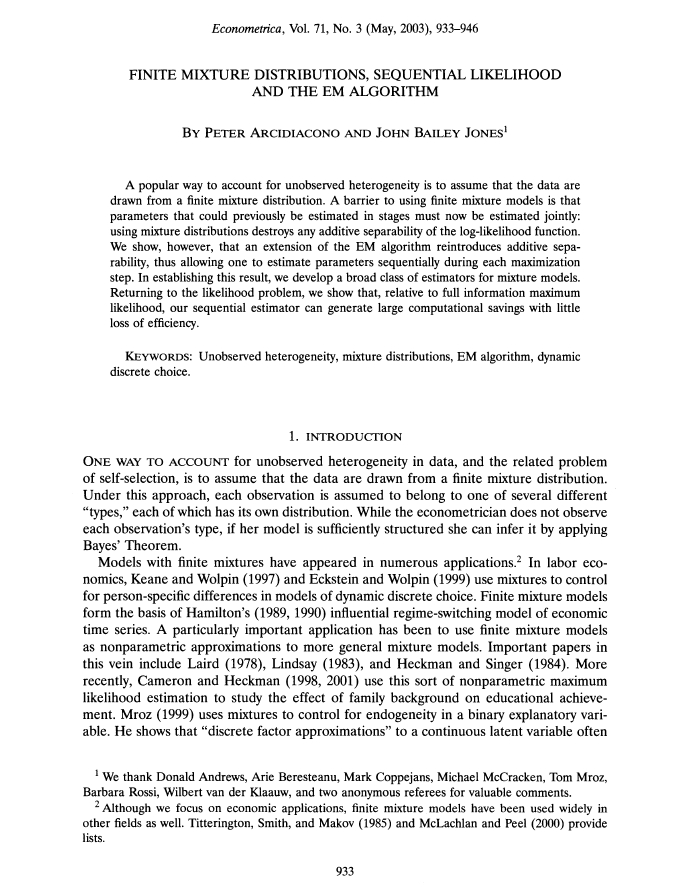
\includegraphics[width=.45\textwidth]{arcidi_jones_cover.jpg}
\end{frame}



\begin{frame}

We can get additive separability of the finite mixture model with the \textcolor{navy}{EM algorithm}

\bigskip

EM stands for ``Expectation-Maximization''

\bigskip

\onslide<2->{
The algorithm iterates on two steps:

\bigskip

\textbf{E-step:} estimate parameters of the mixing distribution (the $\pi$'s)

\bigskip

\textbf{M-step:} pretend you observe the unobserved variable and estimate the $\alpha$'s
}

\bigskip

\onslide<3->{
The EM algorithm is used in other applications to fill in missing data

\bigskip

In this case, the missing data is the permanent unobserved heterogeneity
}

\end{frame}

\begin{frame}

With the EM algorithm, the non-separable likelihood function

\begin{align*}
\ell = \sum_i \log\left(\sum_s \pi_s \prod_t \mathcal{L}(Y_{1t}|X_{1t},\alpha_1,s) \mathcal{L}(Y_{2t}|X_{2t},\alpha_2,s)\right)
\end{align*}

\onslide<2->{
can be written in a form that is separable:

\begin{align*}
\ell = \sum_i \sum_s q_{is} \sum_t \left\{\ell_1(Y_{1t}|X_{1t},\alpha_1,s) + \ell_2(Y_{2t}|X_{2t},\alpha_2,s)\right\}
\end{align*}

where $q_{is}$ is the (posterior) probability that $i$ belongs to group $s$
}

\bigskip

\onslide<3->{
$q_{is}$ satisfies $\pi_s = \frac{1}{N}\sum_{i}q_{is}$
}

\end{frame}

\begin{frame}

We can now estimate the model in stages because of the restoration of separability

\bigskip

The only twist is that we need to \textcolor{navy}{weight} by the $q$'s in each estimation stage

\bigskip

\onslide<2->{
\textbf{Stage 1 of M-step:} estimate $\ell(Y_{1t}|X_{1t},\alpha_1,s)$ weighting by the $q$'s

\bigskip

\textbf{Stage 2 of M-step:} estimate $\ell(Y_{2t}|X_{2t},\alpha_2,s)$ weighting by the $q$'s
}

\bigskip

\onslide<3->{
\textbf{E-step:} update the $q$'s by calculating
$$q_{is} = \frac{\pi_s\prod_t\mathcal{L}(Y_{1t}|X_{1t},\alpha_1,s)\mathcal{L}(Y_{2t}|X_{2t},\alpha_2,s)}{\sum_m\pi_m\prod_t\mathcal{L}(Y_{1t}|X_{1t},\alpha_1,m)\mathcal{L}(Y_{2t}|X_{2t},\alpha_2,m)}$$
}

\onslide<4->{
Iterate on E and M steps until the $q$'s converge
}

\end{frame}

\begin{frame}

With permanent unobserved heterogeneity, we no longer have \textcolor{navy}{global concavity}

\bigskip

\begin{itemize}
    \item This means that different starting values will give different estimates
\end{itemize}

\bigskip

\onslide<2->{
Another issue is \textcolor{navy}{standard errors}
\bigskip

}

\begin{itemize}
    \item<3-> With stages, each stage introduces estimation error into the following stages
    \item[]<4->
    \item<4-> We take the estimate as given, but it's actually subject to sampling error
\end{itemize}
\bigskip

\onslide<5->{
Both issues (local optima and estimation error) are problem-specific

\bigskip

You need to understand your specific case
}

\end{frame}

\end{document}